%%---------------------------------------------------------------------
% 
% Infos
%   Last Modif: 14/10/15
%   Authors: Thomas Moreau,
%
%%---------------------------------------------------------------------


%----------------------------------------------------------------------------------------
%	PACKAGES AND THEMES
%----------------------------------------------------------------------------------------
\documentclass{beamer}
\mode<presentation> {
\usetheme{PrezCMLA}
\usecolortheme{PrezCMLA}
\setbeamertemplate{navigation symbols}{} % Remove the navigation symbols
}

\usepackage{graphicx}
\graphicspath{{../img/}}
\usepackage[utf8]{inputenc}
\usepackage[frenchb]{babel}

\setbeamertemplate{bibliography item}{}
\setbeamertemplate{bibliography entry title}{}
\setbeamertemplate{bibliography entry location}{}
\setbeamertemplate{bibliography entry note}{}
\bibliographystyle{apalike}


\def\mycite#1{\hfill\textcolor{gray}{\cite{#1}}}


% This is only here to get pla highlighting
\AtBeginSection[]
{
 \begin{frame}<beamer>
 \frametitle{Plan}
 \tableofcontents[currentsection]
 \end{frame}
}

%----------------------------------------------------------------------------------------
%	PRESENTATION INFO
%----------------------------------------------------------------------------------------

\title[Debrief NIPS]{Asynchronous Parallel Greedy\\Coordinate Descent}

% Presentation info
\author{Thomas Moreau} % Your name
\institute[CMLA]{ENS Paris-Saclay - CMLA} 
\date{15/10/15} % Date, can be changed to a custom date

% Custom footline
\event{MLMDA Seminar group}
\location{Cachan, FRANCE}


% Add collaborators
%\collaborators{J. Doe}
% ou
%\collaborators[collab]{J. Doe}

% Add supervisor
%\collaborators[supervised]{J. Doe, J. Smith}

% Title for a single frame
% The box around the title can be adapted with the \SizeTitleBox option
\setbeamertemplate{title page}[frame]
\setlength\SizeTitleBox{.8\textwidth}

% Title in a header for the first slide
%\setbeamertemplate{title page}[header]

%----------------------------------------------------------------------------------------
% PRESENTATION
%----------------------------------------------------------------------------------------


\begin{document} 

\begin{frame}[t]
\titlepage 
\end{frame}


\begin{frame}{NIPS interesting papers}
	Presenting 1 paper:\\[.5em]
	\begin{itemize}
		\item Asynchronous Parallel Greedy Coordinate Descent\\
		{\scriptsize \it You, Lian, Liu, Yu, Dhillon, Demmel, Hsieh}\\[1em]
	\end{itemize}
	
	Other interesting papers:
	\begin{itemize}\itemsep.5em
		\item Learning brain regions via large-scale online structured sparse dictionary-learning,
		{\scriptsize \it Dohmatob, Mensch, Varoquaux and Thirion}
		\item Fast and Provably Good Seedings for $k$-Means \\
		{\scriptsize \it {Bachem, Lucic, Hassani and Krause}}
		\item Stochastic Optimization for Large-scale Optimal Transport \\
		{\scriptsize\it Genevay, Cuturi, Peyr{\'e} and Bach}
		\item \dots
	\end{itemize}
\end{frame}

\begin{frame}{Coordinate descent}

	Objective:
	\[
		\min_{x\in\Omega} f(x)
	\]
	with $\Omega \subset \mathbb R^N$, and $f$ smooth and convex.\\[2em]
	
	{\bf Classic approach:} projected gradient descent
	\[
		x_{k+1} = \mathcal P_\Omega\left(x_k - \alpha \nabla f(x_k) \right)
	\]\\[1em]
	
	{\bf A subgradient approach:} coordinate descent \mycite{friedman2007pathwise}
	\[
		x_{k+1} = \mathcal P_\Omega\left(x_k - \alpha \nabla_{i_k} f(x_k) \right)
	\]
	
	with $\alpha > 0$ 
	 
\end{frame}
\begin{frame}{Coordinate descent - Stochastic versus Greedy}
	\onslide<+->{Big question with coordinate descent: {\bf How do you choose $i_k$?}}\\[1.5em]
	
	\begin{itemize}[<+->]\itemsep1em
	\item {\bf Cyclic updates:} inefficient,\mycite{friedman2007pathwise}
	\item {\bf Random updates:} low computational complexity, good convergence,
	\item {\bf Greedy updates:} better convergence, higher computational complexity.\mycite{li2009coordinate}\\
	$\Rightarrow$ Problem dependent! Usefull for instance with SVM and LASSO.
\end{itemize}
\onslide<+->{Coordinate Descent Converges Faster with the \\
Gauss-Southwell Rule Than Random Selection \mycite{nutini2015coordinate}
\[
	\mathbb E\left[f(x_{k+1})\right] - f(x^*) < \begin{cases}
		\left(1- \frac{\mu}{nL}\right)\left(f(x_k) - f(x^*)\right) &\hfill\textcolor{gray}{Random}\\[.5em]
		\left(1- \frac{\mu_1}{L}\right)\left(f(x_k) - f(x^*)\right) & \hfill\textcolor{gray}{GS}
		\end{cases}
\]
}
	
	
\end{frame}
%\begin{frame}{Coordinate descent - properties}
	
%\end{frame}
\begin{frame}{Parallel asynchronous approaches}

{\bf Basic idea:} Update simultaneously and independently the coordinates.\\[1em]

\begin{itemize}\itemsep.5em
	\item Passcode: Parallel asynchronous stochastic dual coordinate descent\\\mycite{hsieh2015passcode}\\
	\item An asynchronous parallel stochastic coordinate descent algorithm \\\mycite{liu2015asynchronous}\\
	\item Asynchronous Parallel Greedy Coordinate descent \\$\rightarrow$This paper! \mycite{you2016asynchronous}\\
	\item \dots

\end{itemize}

\end{frame}

\begin{frame}{The algorithm}
	Let $\left \{ S_i \right \}_{i=1\dots n} $ a non-overlapping partition of $\left \{ 1\dots N \right \}$.\\
	In parallel on all cores:\\[.7em]
\begin{itemize}\itemsep1em
	\item Randomly select $S_k$  and choose $i_k = \arg\max_{i \in S_k} \|\nabla^+_if(\widehat x)\|$ 
	\item Update $x_{k+1} = \mathcal P_\Omega\left( x_k - \gamma \nabla_{i_k} f(\widehat x_k)\right)$ 
\end{itemize}
with \[
	\nabla_{i_k}^+f(\widehat x_k) = x_k - \mathcal P_\Omega\left(x_k - \nabla_{i}^+f(\widehat x_k) \right)
\]

{\color{gray} This should be:
\[
	\nabla_{i_k}^+f(\widehat x_k) = \widehat x_k - \mathcal P_\Omega\left(\widehat x_k - \nabla_{i}^+f(\widehat x_k) \right)
\]as $x_k$ is not known because of {\bf inconsistent read}.
}
	
\end{frame}

\begin{frame}{Theoretical result}

{\bf Assumptions}
\begin{enumerate}\itemsep1em
	\item {\bf Bounded Delay:} $x_k$ and $\widehat x_k$ differs on at most $T$ coordinates.
	\item {\bf Lipschitz gradient :} $\forall x, y~~ \|\nabla f(x) - \nabla f(y)\| \le L \|x-y\|$
	\item {\bf Global error bound:} when $\gamma = \frac{1}{3L_{max}}$, $\exists \kappa > 0$ s.t.:
	\[
	   \|x - \mathcal P_S(x)\| \le \kappa\|x-\widetilde x\|
	\]
	where $\widetilde x = \arg\min_{y \in \Omega} \langle \nabla f(x), y-x \rangle + \frac{1}{2\gamma}\|y-x\|^2$ and\\ $S$ is the set of optimal solutions.
	\item All random variables in $\left \{ S_k \right \}_{k=1\dots K}$ are independent to each other
\end{enumerate}
	
\end{frame}

\begin{frame}{Theoretical result}

{\bf Theorem:}
\begin{itemize}
	\item[] Choose $\gamma = \frac{1}{3L_{max}}$, suppose $n \ge 6$ and that the staleness $T$ verify:
	\[
		T(T+1) \le \frac{\sqrt n L_{max}}{4eL_{res}}
	\] 
	\item[] Then
	\[ 
		\mathbb E(f(x_k) - f^*) \le \left(1 - \frac{2L_{max}b}{L\kappa^2n}\right)^k ( f(x_0) - f^*)
	\]with $b = \left(\frac{L_T^2}{18 \sqrt n L_{max} L_{res}}+ 2\right)^{-1}$ 
\end{itemize}

	
\end{frame}

\begin{frame}{Their numerical results}
{\bf Application to Multi-core kernel SVM\\[1em]}
Dataset: $\left \{ a_i \right \}_{i=1}^l$ and corresponding labels $y_i\in \left \{ +1, -1 \right \}$
\[
\min_{\alpha\in\mathbb R^N} \frac{1}{2} \alpha^TQ\alpha - {\bf 1}^T\alpha ~~~~s.t~~~~ 0 \le \alpha \le C
\]
where $Q \in y^TKy$\\[1em]

{\bf Update rule: $\delta^*_i = \mathcal P_{\left[0, C\right]}(\alpha_i - \frac{\nabla_if(\alpha)}{Q_{ii}})-\alpha_i$}\\[.5em]
{\color{gray}Note that $\gamma = \frac{1}{Q_{ii}}$ as it gives $\delta^*_i = \arg\min_\delta f(\alpha + \delta e_i)$ }\\[1em]

Efficient as $g = \nabla f(\alpha) = Q\alpha - {\bf 1}$ can be maintained cheaply:
\[\alpha = \alpha + \delta_i \rightarrow g = g + \delta_iq_i \] 
	
\end{frame}

\begin{frame}{Their numerical results}

	{\bf Setting:}
	\begin{itemize}\itemsep1em
	\item Single machine with 20 cores and 256GB of shared memory, using 2 sockets.
	\item Comparison with LibSVM and Asy-SCD.
	\item Use kernel caching with LRU implementation on each core.
	\item 3 classical datasets for SVM ({\tt ijcnn1, covtype, webspam}).
	\item Extra clusterization to avoid big interference. \mycite{Scherrer2012}
	\item Partition $\left \{ S_i \right \}_{i=1\dots n} $ with $n$ been the number of cores.
\end{itemize}
	
\end{frame}
\begin{frame}{scale up}

\begin{figure}[htp]
\centering
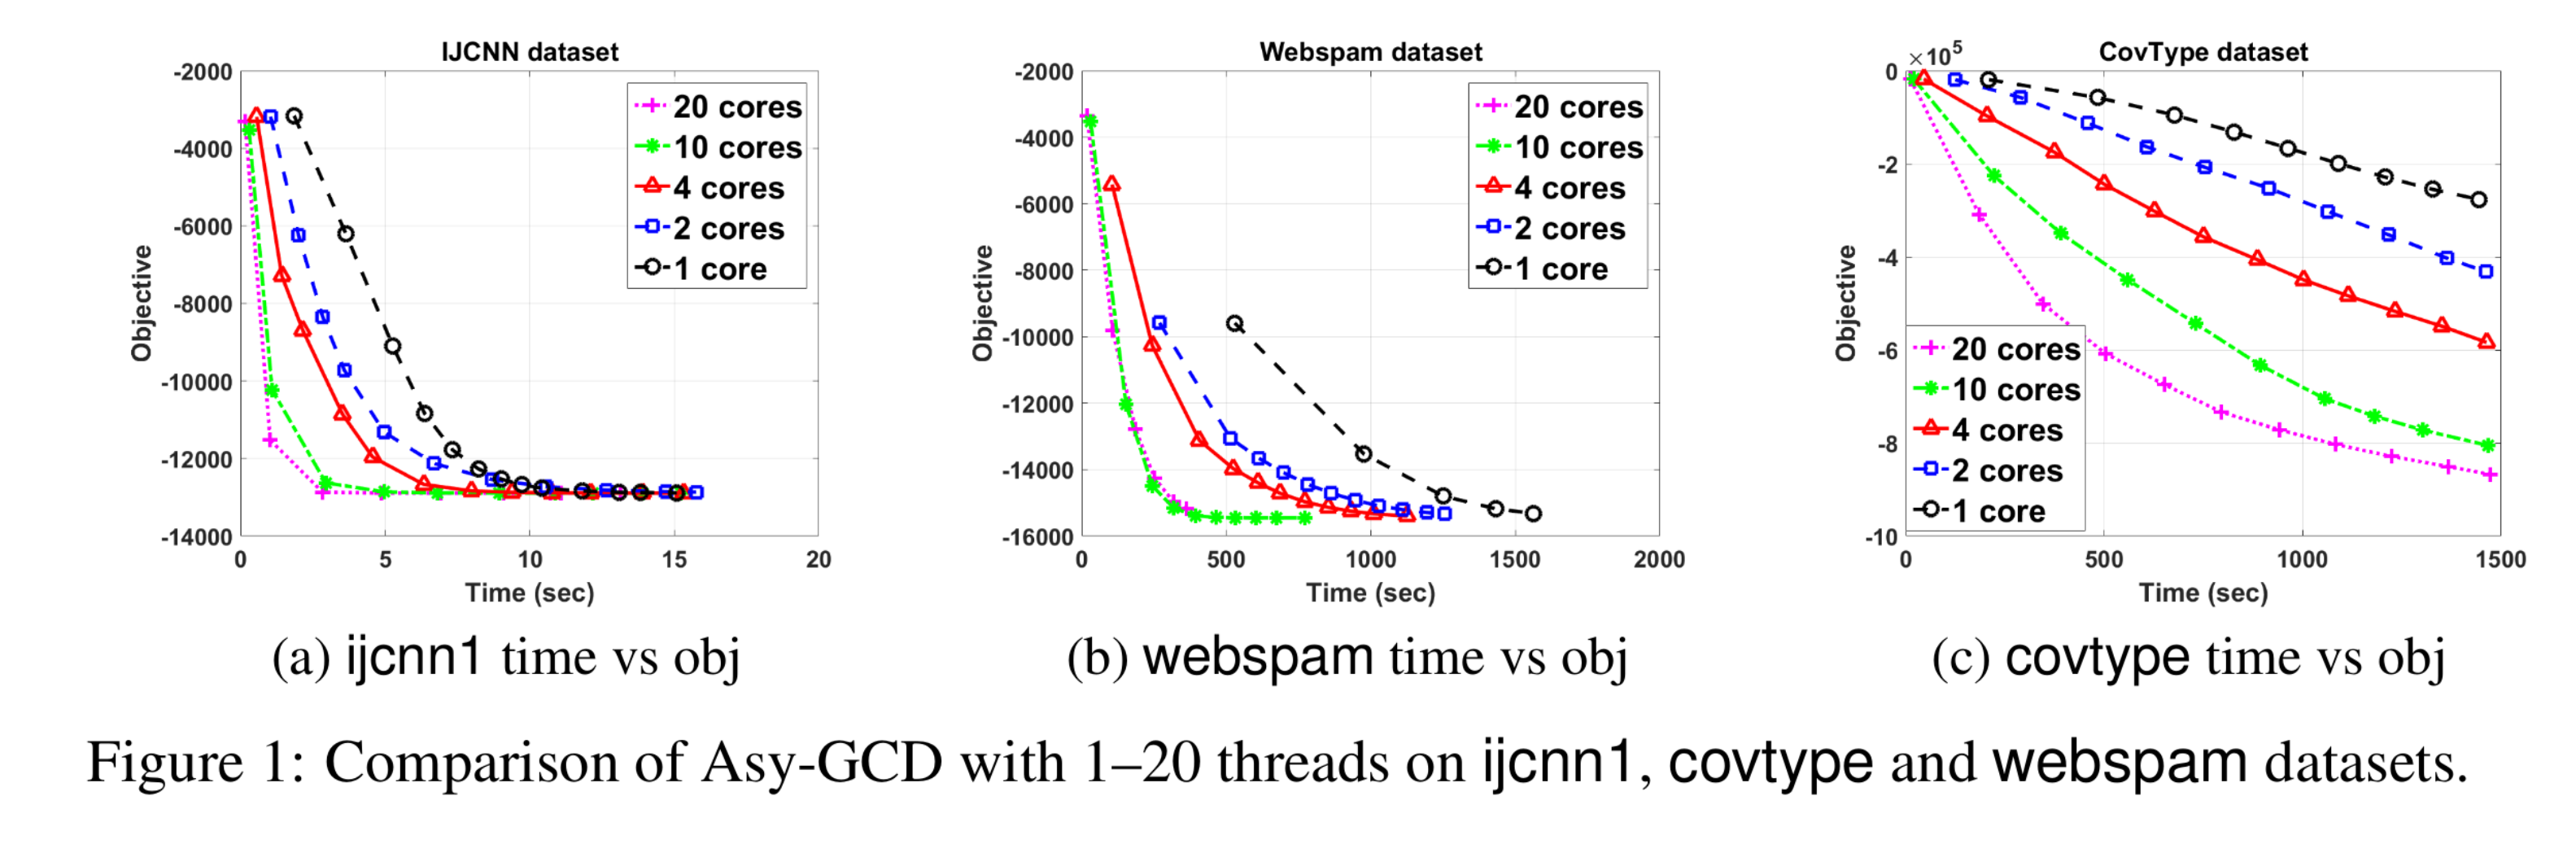
\includegraphics[width=\textwidth]{fig1}\\[-.2em]
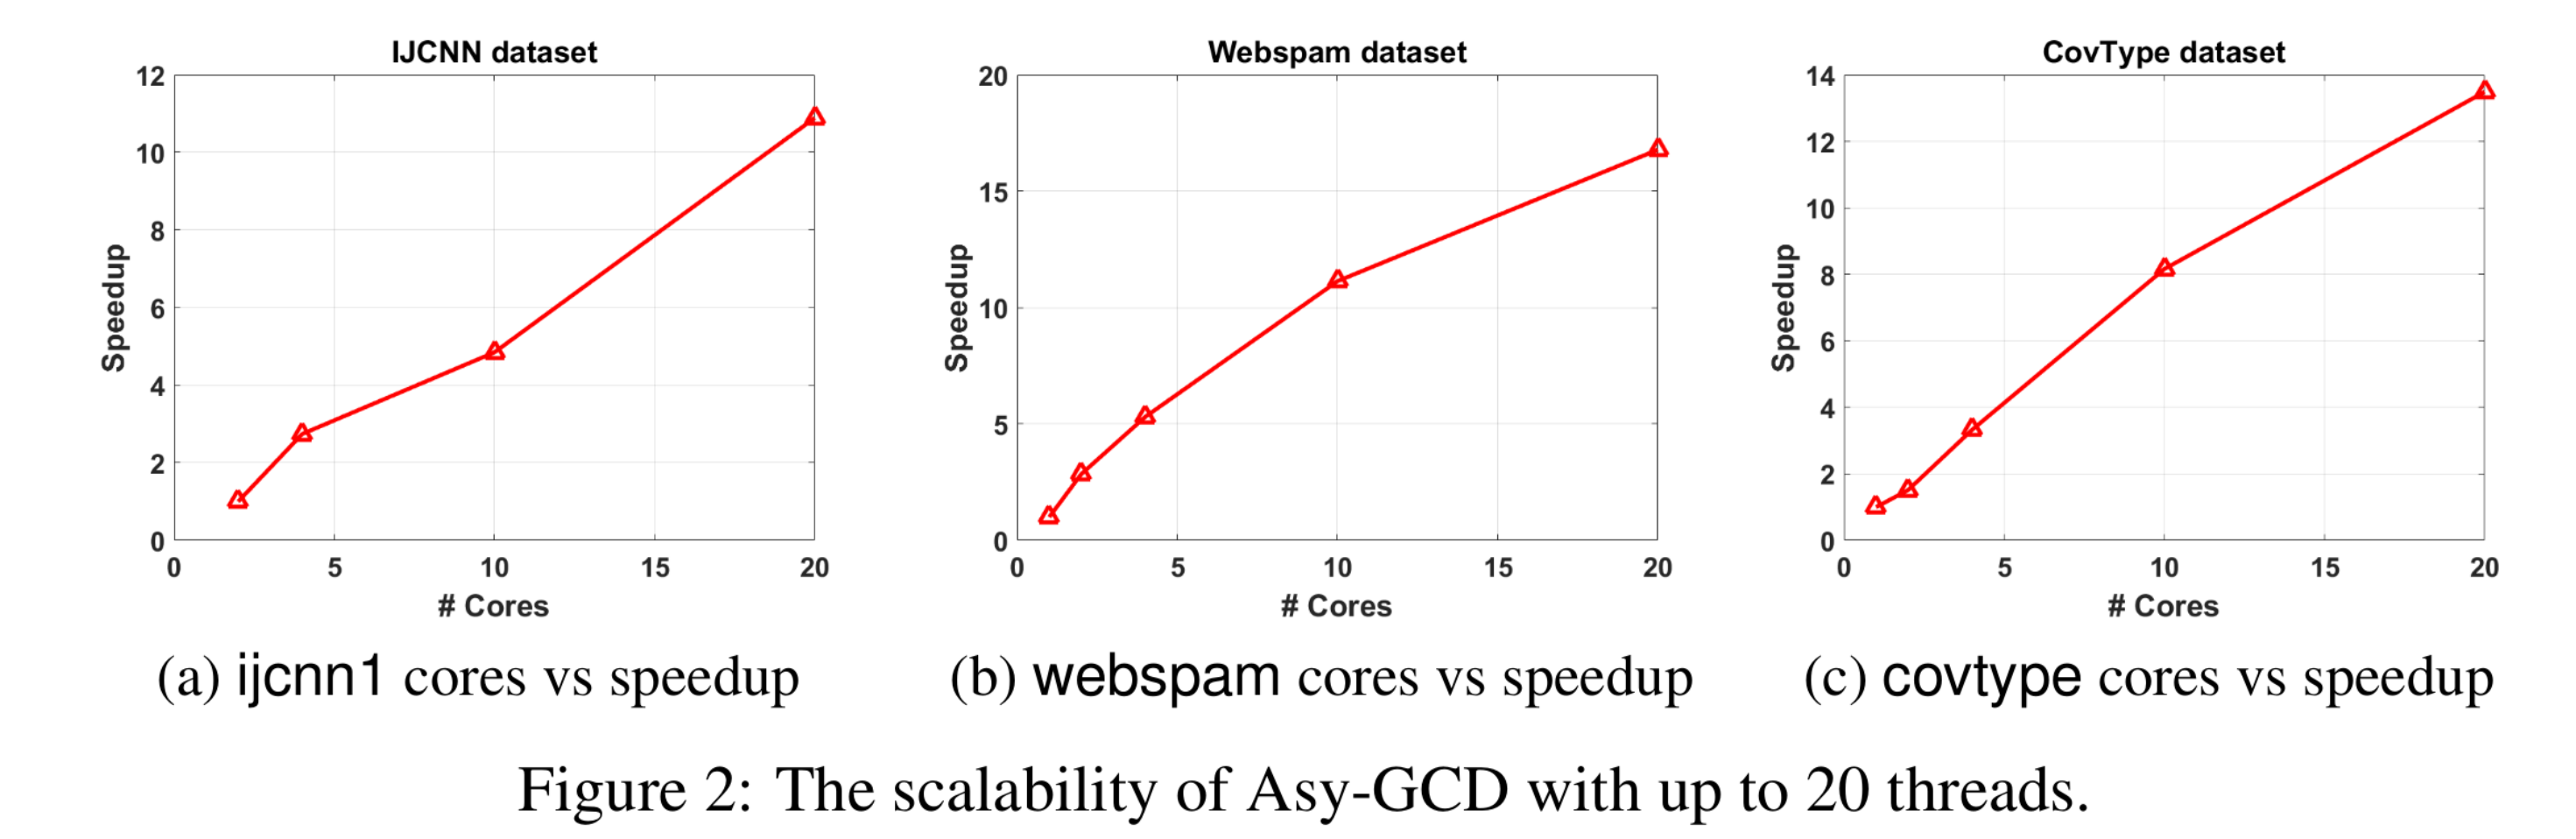
\includegraphics[width=\textwidth]{fig2}
\end{figure}

	
\end{frame}
	
\begin{frame}{Comparison to other solver}

\begin{figure}[htp]
\centering
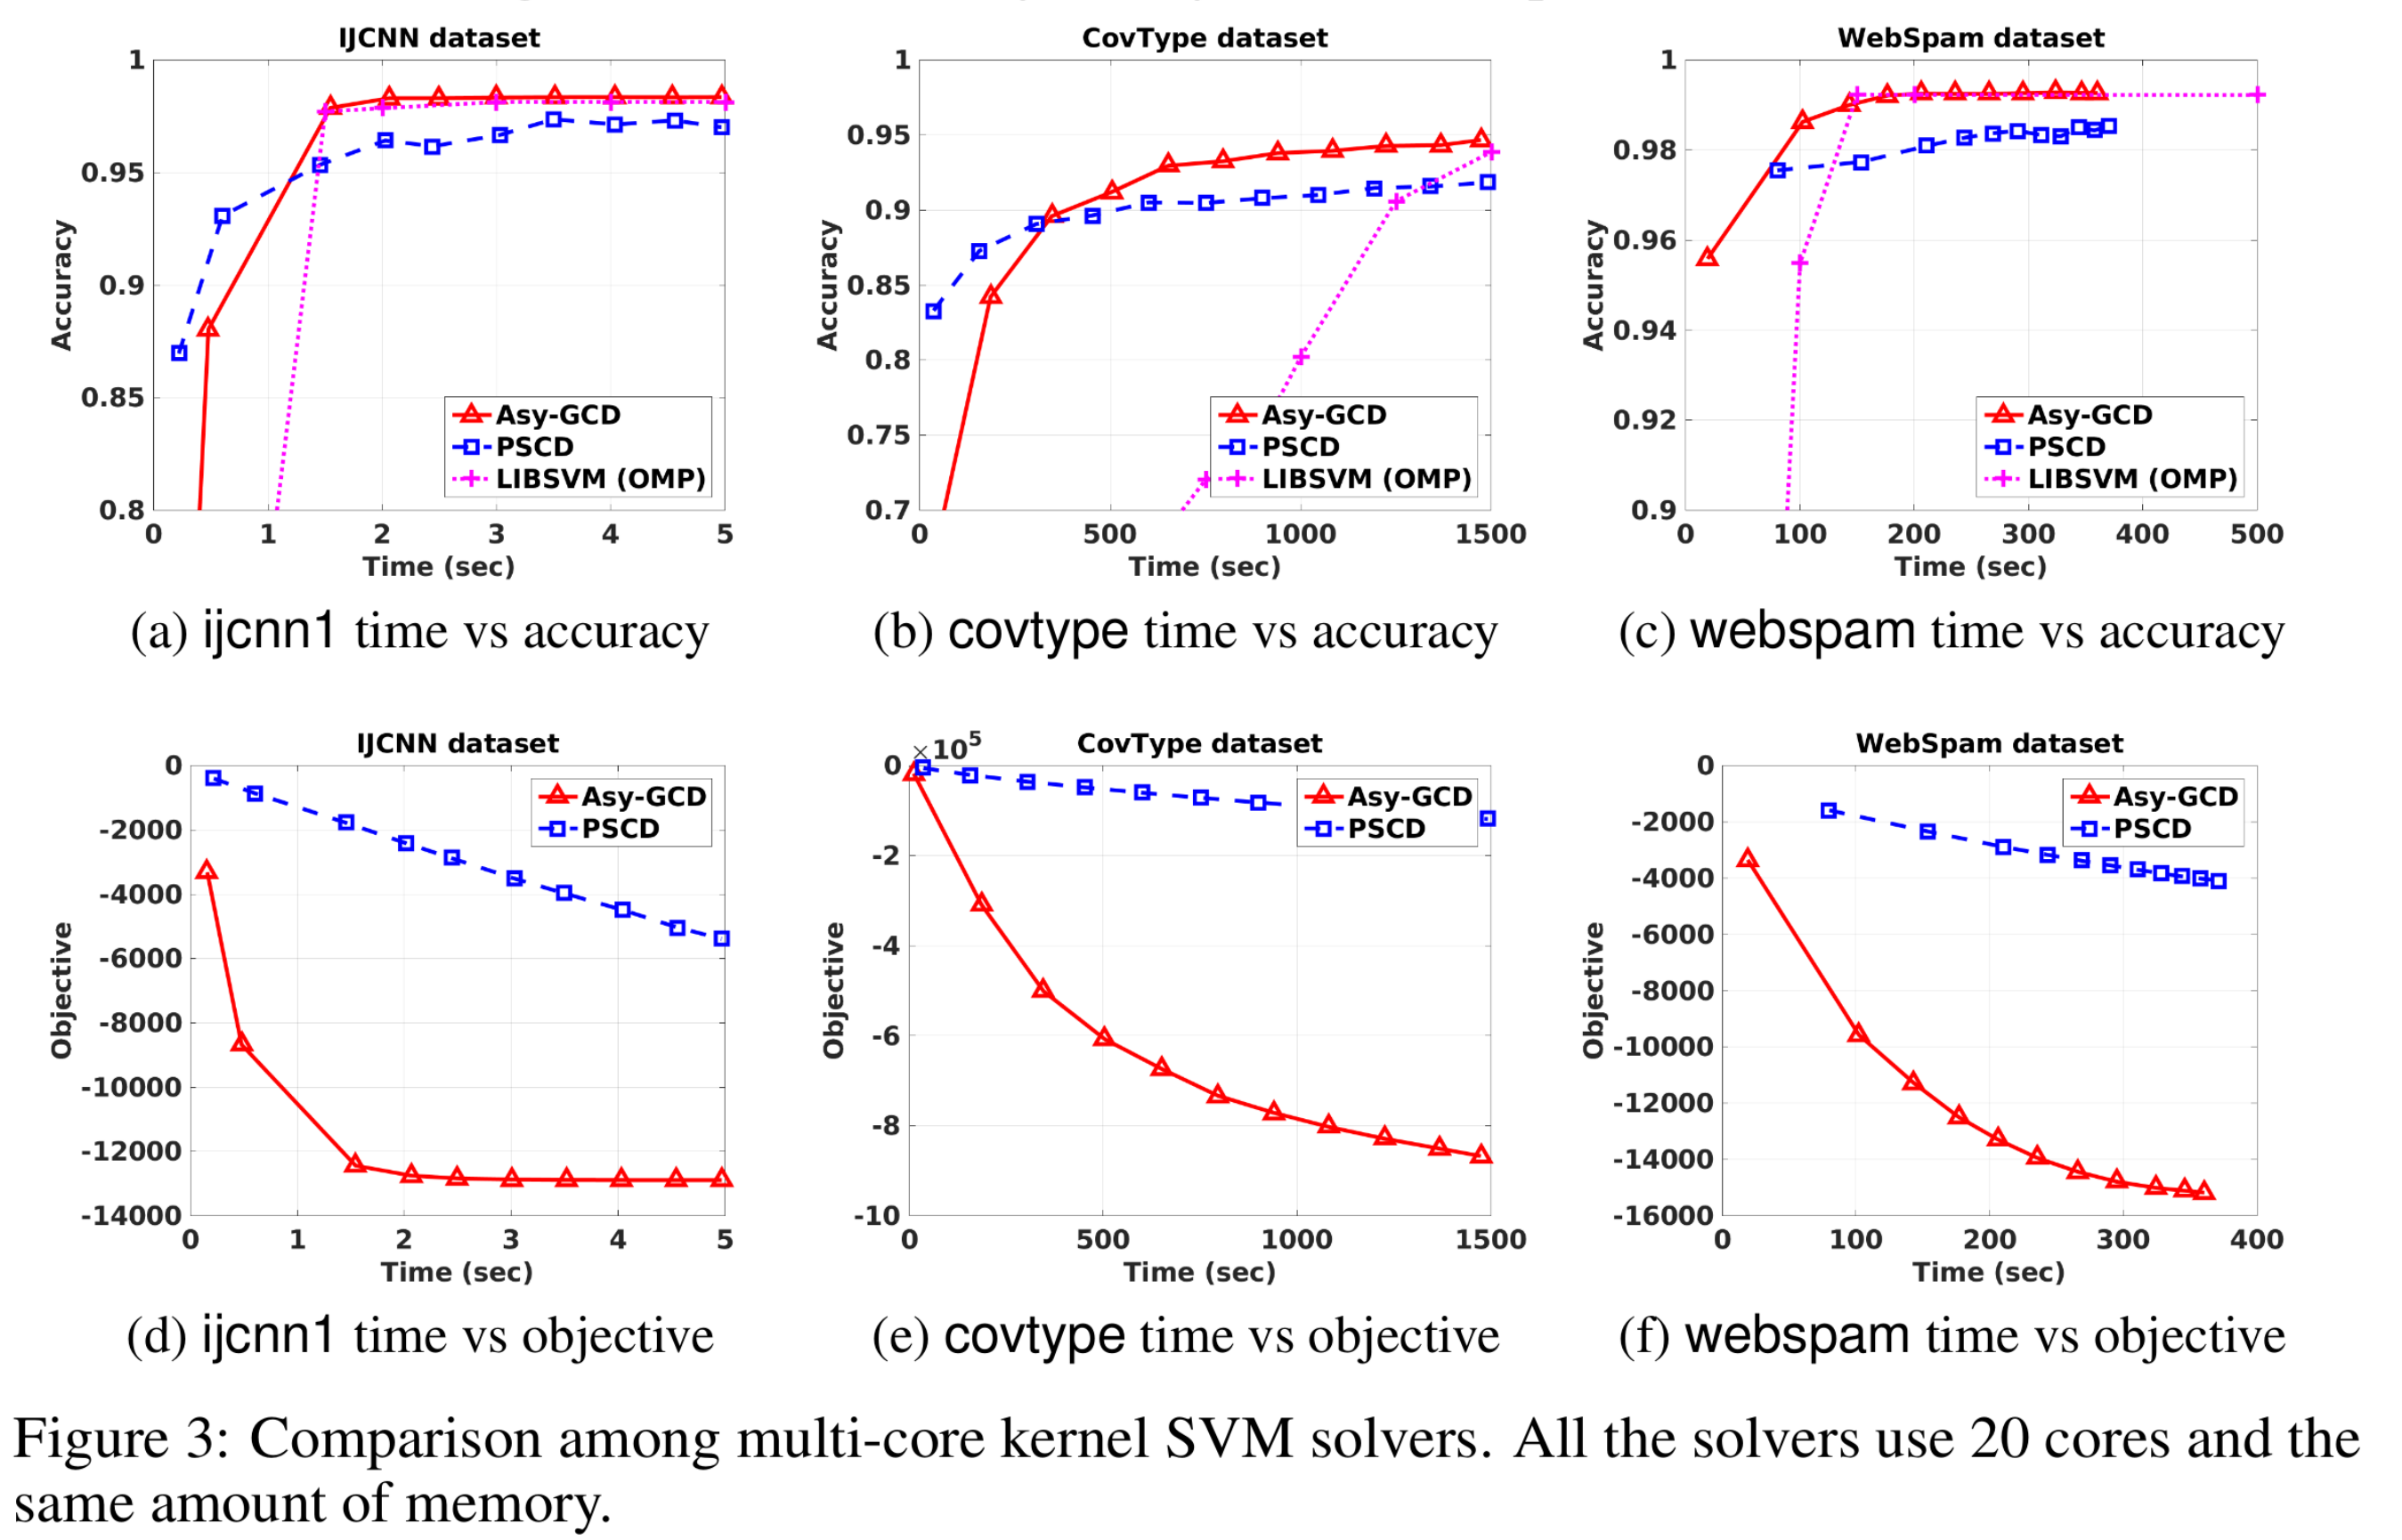
\includegraphics[width=\textwidth]{fig3}
\end{figure}
\end{frame}

\begin{frame}{Conclusion}

\begin{itemize}\itemsep1em
	\item Interesting framework to study greedy asynchronous CD.
	\item Lack of intuition (and proof) for the theoretical aspect.
	\item Weird setup for the numerical experiments.
\end{itemize}
	
\end{frame}


\begin{frame}
\begin{center}

\Huge Questions?
	
\end{center}
	
\end{frame}
%--------------------------------------------------------------------------
% REFERENCES
%--------------------------------------------------------------------------

\begin{frame}[noframenumbering]{References}
	\nocite{*}
	\tiny\bibliography{lib}
\end{frame}


\end{document} 